\begin{figure*}[ht]
  \centering
  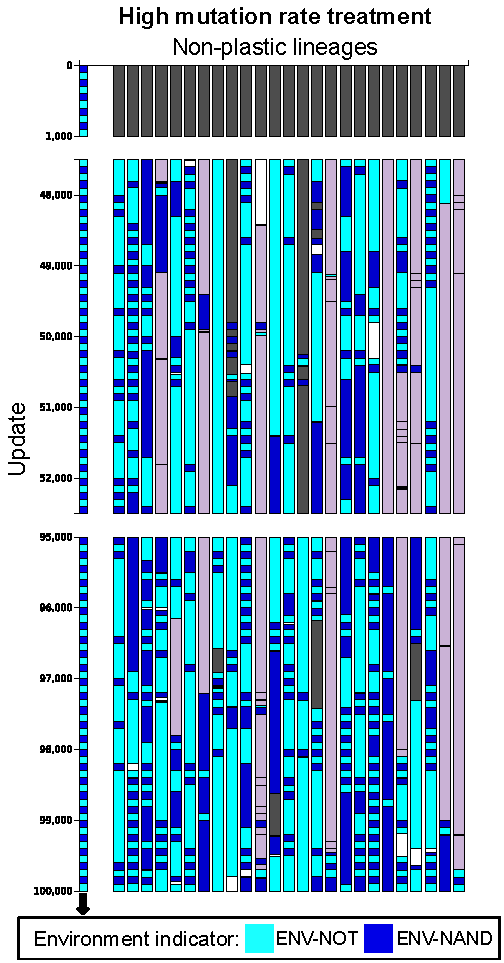
\includegraphics[height=0.5\textheight, keepaspectratio]{chapters/02-evolutionary-origins-of-plasticity/media/high-mutation-rate-non-plastic-lineages.pdf}
  \caption{\small 
  Time-sliced visualization of lineages for non-plastic, dominant genotypes from the high-mutation-rate treatment. 
  Abbreviated color reference: 
  cyan represents unconditional NOT task performance, 
  dark blue represents unconditional NAND task performance, 
  and light purple represents sub-optimal forms of plasticity.  
  Refer to Figure \ref{chapter:origins-of-plasticity:fig:task-profiles} for a full legend of phenotype colors.}
  \label{chapter:origins-of-plasticity:fig:high-mut-lineages}
\end{figure*}

